\chapter{Signaling and scrambling with strongly long-range interactions}
In non-relativistic quantum mechanics, Lieb-Robinson bounds provide a notion of causality \cite{LR}, limiting the speed of information propagation (or signaling) to a finite value in lattice systems with short-range interactions. This bounded signaling speed has strong implications for quantum information and condensed matter physics, leading to entanglement area laws \cite{Hastings07} and the existence of topological order \cite{BravyiHM10}.
\red{However, it remains an open question whether the signaling speed must be finite if interactions are long-ranged and decay as an inverse power-law $1/r^{\al}$ in the inter-particle distance $r$.}
Such power-law interacting systems arise in experimental platforms for quantum computation and quantum simulation, including Rydberg atoms ~\cite{Saffman10}, trapped ions~\cite{Britton12}, polar molecules~\cite{Yan13}, defect centers in solids~\cite{Yao12}, and atoms trapped along photonic crystals~\cite{Douglas15}.
% The lack of a bounded signaling speed in these systems makes it challenging to understand and predict their dynamics.
For $D$-dimensional power-law interacting systems with $\al$ greater than $2D+1$, a finite signaling speed has been shown \cite{Chen2019,kuwaharaStrictlyLinearLight2020}.

% At long distances (or times), recent developments show that the signaling speed will diverge at most polynomially in time for $\al >2D$ \cite{Foss-Feig15, Tran18}, ruling out the exponential divergence suggested by earlier results \cite{HK}.
% For $\al\le 2D$, which is the case for most experimental long-range interacting systems, an exponentially growing signaling speed has yet to be ruled out, making the fate of causality far from settled.

In this work, we focus on the regime of \emph{strongly long-range} interacting systems, where interaction energy per site diverges, thus implying $\al\le D$ \cite{Kastner11,Kastner12, Storch15, Kastner17}.
Note that even if one normalizes the interaction strength to make energy \emph{extensive} (i.e., proportional to the number of lattice sites), these systems are still fundamentally different from those with $\al >D$ (as energy is in general no longer additive for subsystems \cite{Dauxois}).
To avoid confusion, we will not perform any normalization of interaction strength throughout this paper, as such normalization can be performed later by rescaling time  without changing the physics implied by our results \cite{Storch15}.

Apart from their existence in experimental platforms \cite{Monroe13, Britton12, Blatt12,Yan13,Lukin17}, strongly long-range interacting systems have received much theoretical interest due to their applications in spin squeezing \cite{FossFeig16}, novel behavior in dynamical critical scaling \cite{Defenu18,Acevedo14}, divergent equilibration time \cite{Kastner11}, and close relation to fast quantum-information scrambling \cite{SY93,Bollinger17, Kitaev15, Maldacena16, SS08,Lucas18,Lucas19}. The phenomenology of these systems differs from that of their short-range counterparts at a fundamental level, and thus require new theoretical understandings.
Two fundamental questions about these systems are (1) what is the shortest time $t_{\text{si}}$ needed to send a signal from one site to a site located an extensive distance away, and (2) what is the shortest time $t_{\text{sc}}$ needed to scramble the information stored in the system \footnote{We will define the quantities $t_{\text{si}}$ and $t_{\text{sc}}$ rigorously later in the paper}?

There have been a number of attempts to answer the above two questions, with limited success.
For the first question, Refs.~\cite{Eisert13,Hauke13,Eldredge17} show that in certain strongly long-range interacting systems with $\alpha\le D$, information and correlations can spread across the entire system in a finite time that is independent of the number of sites, $N$.
(For certain systems not engineered for fast signaling or scrambling, information propagation may even be suppressed~\cite{Santos16}.)
The Lieb-Robinson-type bound derived in Ref.~\cite{Storch15}, however, suggests that the signaling time can vanish in the $N\rightarrow\infty$ limit, and does not rule out the possibility of $t_\text{si}$ scaling as $\log(N)\,N^{2\alpha/D}/N^2$ for $\alpha < D$.
No protocol that we know of comes close to achieving such fast signaling.
As for scrambling, Ref.~\cite{Lashkari13} shows that the scrambling time can be lower-bounded by  $t_\text{sc} \gtrsim 1/N$ for $\alpha=0$, whereas the fastest-known scramblers are conjectured to be able to scramble in time $t_\text{sc} \propto \log(N)/\sqrt{N}$\ \cite{SS08}.

While the definitive answers to these two questions remain to be found, we present several advances in this paper.
First, we prove a new bound for systems that can be mapped to free bosons or fermions with $1/r^{\alpha}$ hopping strength, which leads to a signaling-time bound of $t_\text{si} \gtrsim N^{\alpha/D}/\sqrt{N}$.
While no previous bound has been given specifically for free-particle systems, the best existing result for interacting systems yields a significantly looser bound of $t_\text{si} \gtrsim \log(N)\,N^{2\alpha/D}/N^2$~\cite{Storch15}
\footnote{While the original bound in Ref.~\cite{Storch15} was stated in terms of $n$-body interactions, here we cite the bound on the interaction time as it applies to the specific case of two-body interactions.}.
Notably, our free-particle bound is tight for $\alpha\le D/2$, as we show that it can be saturated by a new quantum state transfer protocol.

We also prove a bound of $t_{\text{si}}\gtrsim \log(N)N^{\alpha/D}/N$ for general interacting spin systems, which\dash while improving significantly over the previous best bound mentioned above~\cite{Storch15}\dash is still not known to be tight.
Building on this second result, we prove a tight bound for ``many-site signaling'' (from one site to an extensive part of the system).
This many-site signaling bound leads to a scrambling-time bound of $t_\text{sc}\gtrsim N^{\alpha/D}/N$, which generalizes the result in Ref.~\cite{Lashkari13} of $t_\text{sc} \gtrsim 1/N$ to all $\alpha<D$.

\sect{Tight bound for free particles}We first prove a Lieb-Robinson-type bound for non-interacting bosons/fermions on a lattice. Consider the following free-particle Hamiltonian $H(t)$ defined on a $D$-dimensional lattice $\Lambda$ with $N$ sites:
 \begin{equation}
    \label{eq:freeHam}
 	H(t) = \sum_{\substack{i,j\in\Lambda \\ i< j}} (J_{ij}(t) c_i^\dagger c_j + \text{h.c.}) + \sum_{i\in\Lam}B_{i}(t)c_i^\dagger c_i,
    \end{equation}
where $c_i^\dagger$ ($c_i$) represents the creation (annihilation) operator. The hopping strength $J_{ij}(t)$ and chemical potential $B_i(t)$ can depend on time and we do not impose any constraint on them for now. We denote an operator $A$ at time $t$ in the Heisenberg picture as $A(t)=U^\dagger(t)A U(t)$, where $U(t) \equiv \mathcal{T} e^{-\frac i \hbar \int_0^t H(t')\,dt'}$ is the time evolution operator ($\hbar = 1$). The operator norm of $A$ will be denoted by $\|A\|$.
\begin{theorem}
    \label{eq:tightbound}
For the Hamiltonian defined in \cref{eq:freeHam} and any pair of distinct sites $X, Y \in \Lam$,
\begin{equation}
    \label{eq:tightboundeq}
    \left\Vert \left[c_{X}(t),c_{Y}^{\dagger}\right]\right\Vert \le  \int_{0}^{t}d\tau\sqrt{\sum_{i\in\Lambda}\left|J_{iX}(\tau)\right|^{2}}.
\end{equation}
\end{theorem}
We use $[\cdot,\cdot]$ to denote the commutator for bosons and anti-commutator for fermions.

Roughly speaking, the quantity $\|[c_{X}(t),c_{Y}^{\dagger}]\|$ measures the overlap between the support of the operator $c_{X}(t)$ (which expands from site $X$ due to hopping terms) and the site $Y$.
As a result, it also quantifies the amount of information that can be sent between $X$ and $Y$ in a given time $t$.
Indeed, we define the signaling time $t_\text{si}$ as the minimal time required to achieve $\|[c_{X}(t),c_{Y}^{\dagger}]\| > \delta$ for some positive constant $\delta$.
Note that we do not expect the chemical potential strength $B_i(t)$ to show up in the bound, as on-site Hamiltonian terms do not change the support of $c_X(t)$.

If the hopping terms in the Hamiltonian are short-ranged (e.g., nearest-neighbor), one might expect $\|[c_{X}(t),c_{Y}^{\dagger}]\|$ to decay exponentially in the distance $r_{XY}$ between $X$ and $Y$, due to the strong notion of causality that follows from the Lieb-Robinson bound \cite{LR}.
Additionally, if the hopping strength decays as a power law ($|J_{ij}(t)|\le 1/r^{\alpha}$) with $\alpha>D$, intuition would suggest that $\|[c_{X}(t),c_{Y}^{\dagger}]\|$ decays algebraically in $r_{XY}$ \cite{HK,Gong14}, indicating a weak notion of causality.
However, the right-hand side of \cref{eq:tightboundeq} has no dependence on $r_{XY}$.
This is because the bound is tailored to strongly long-range hoppings with $\alpha<D$, which makes it loose for shorter-ranged long-range hoppings.

Assuming that $|J_{ij}(t)|\le 1/r^{\alpha}$, we can simplify \cref{eq:tightboundeq} to
\begin{equation}
\left\Vert \left[c_{X}(t),c_{Y}^{\dagger}(0)\right]\right\Vert \le t\times\begin{cases}
\O{1} & \al > D/2,\\
\O{N^{\frac{1}{2}-\al/D}} & 0\le \al\le D/2.
\end{cases}\label{eq:corollary}
\end{equation}
where $N$ is the number of lattice sites and $\mathcal{O}$ is the asymptotic ``big-$\mathcal{O}$'' notation \cite{bigO}. Therefore, for $\al\le D/2$, it takes a time $t_\text{si} = \W{N^{\alpha/D}/\sqrt{N}}$ \cite{bigO} to signal from site $X$ to site $Y$, independent of the distance between $X$ and $Y$.

In the next section, we show that for $\alpha\le D/2$, the bound in \cref{eq:tightboundeq} can be saturated (up to a factor of 2) by engineered free-particle Hamiltonians.
This leads to the conclusion that causality can completely vanish\dash in the sense that signals can be sent arbitrarily fast given large enough $N$\dash for a strongly long-range hopping system with $\alpha<D/2$.
It remains an open question whether such a statement can be generalized to systems with $D/2 \le\alpha<D$ for either free or interacting particles.


\sect{Proof of \cref{eq:tightbound}}Let us first go into the interaction picture of $\sum_i B_{i}(t)c_i^\dagger c_i$ to eliminate the on-site terms from the Hamiltonian in \cref{eq:freeHam}.
(This imparts a time-dependent phase $e^{i\phi_{jk}(t)}$ onto the hopping term $J_{jk}(t)$ for some $\phi_{jk}(t)\in[0,2\pi)$ and $j\neq k$, which---since it does not change the value of $|J_{jk}(t)|$---does not affect the overall bound.)
We now have a pure hopping Hamiltonian $ H_I(t) = \sum_{ij} \tilde J_{ij}(t)c_i^\dagger c_j$ with $|\tilde J_{ij}(t)|\equiv|J_{ij}(t)|$.
Because $ H_I(t)$ is a quadratic Hamiltonian, $c_X(t)$ is a time-dependent linear combination of annihilation operators on every site, and we can write $[c_X(t), c^\dagger_Y] \equiv f_{XY}(t) \mathds{1}$, where $f_{XY}(t)$ is a number and $\mathds{1}$ represents the identity operator.
Given that $U_I(t)\ket{\vac}=\ket{\vac}$, where $U_I(t)$ is the time-evolution operator corresponding to $H_I(t)$, and $c_X(t)\ket{\vac}=0$, we have
\begin{equation}
	\label{eq:deffxy}
	f_{XY}(t) = \bra{\vac}[c_X(t), c^\dagger_Y]\ket{\vac} = \bra{\vac} c_X(0)U_I(t)c^\dagger_Y \ket{\vac}.
\end{equation}
For convenience, we define the (normalized) states $\ket{\psi_X} \equiv c^\dagger_X(0)\ket{\vac}$ and $\ket{\psi_Y(t)} \equiv U_I(t)c_Y^\dagger\ket{\vac}$. Taking the time derivative of \cref{eq:deffxy} gives
\begin{equation}
	\label{eq:onelineproof}
	\frac{df_{XY}}{dt} = -i\bra{\psi_X} H_I(t)\ket{\psi_Y(t)}.
\end{equation}
By the Cauchy-Schwarz inequality,
\begin{align}
\left\Vert  \frac{df_{XY}}{dt}\right\Vert &\le \left\Vert H_I(t)\ket{\psi_X} \right \Vert \: \left\Vert \ket{\psi_Y(t)} \right \Vert\\
&=\left\Vert H_I(t)\ket{\psi_X} \right \Vert= \sqrt{\sum_{i\in\Lambda}\left| \tilde J_{iX}(t)\right|^{2}}.
\end{align}
The last equality follows from $\ket{\psi_X}$ being a single excitation localized on site $X$ and $ H_I(t)$ consisting only of hopping terms $\tilde J_{ij}(t)c_i^\dagger c_j$. Applying the fundamental theorem of calculus yields the bound on  $f_{XY}(t)$ and hence \cref{eq:tightbound}.

\begin{figure}
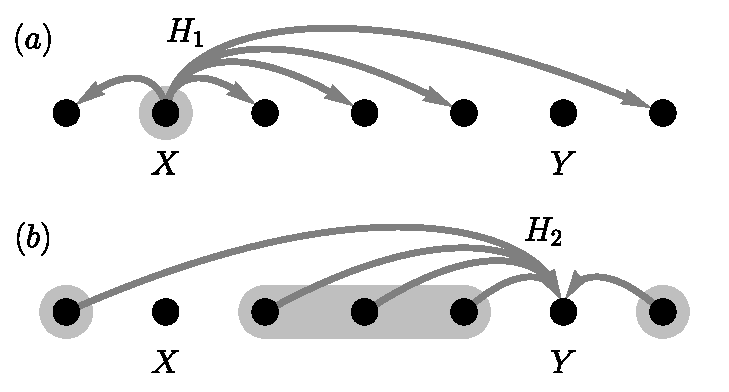
\includegraphics[width=0.9\linewidth]{figures/test_gong_protocol3.pdf}
\caption{A fast quantum state transfer protocol for a long-range Hamiltonian acting on a lattice of dimension $D=1$ with $N=7$ sites. The strengths of the hopping terms are bounded by a power-law $1/r^{\al}$ in the distance $r$. The active interactions in each time-step are depicted as directed edges with uniform weights. (a) The site $X$ is initially in the state $\ket{\psi}$ (gray circle), with the other (unoccupied) sites in state $\ket{0}$. Time-evolving by the Hamiltonian $H_1$ for time $\O{N^{\al/D-1/2}}$  (indicated by gray arrows) yields a superposition of the $\ket{0}^{\otimes N}$ state and a symmetric $\ket{W}$ state over the remaining $N-2$ sites. (b) Applying the Hamiltonian $H_2$ for the same duration of time completes the state transfer of $\ket{\psi}$ to the target site $Y$.}
\label{Fig_Gong}
\end{figure}

\sect{Saturating the free-particle bound}We now show that the bound in \cref{eq:tightbound} can be saturated by engineered Hamiltonians that can also be used to perform fast quantum state transfer. In particular, the protocol presented here has a state transfer time of $T = \O{N^{\alpha/D}/\sqrt{N}}$, which\dash for $\alpha\le D/2$\dash improves over the fastest-known state transfer protocol using long-range interactions \cite{Eldredge17}.

Our setup for the state transfer task is depicted in \cref{Fig_Gong}. We initialize a lattice with $N$ sites in a tensor product of unoccupied states $\ket{0}$ and some unknown normalized bosonic/fermionic state $\ket{\psi} = a\ket{0}+b\ket{1}$ on a single site $X$.
The goal of state transfer is to move $\ket{\psi}$ to the target site $Y$ after the system time-evolves by a $\ket{\psi}$-independent (but possibly time-dependent) Hamiltonian $H(t)$ \cite{NJ2014,Epstein17}.

The unitary time-evolution operator $U(T)$ can be said to implement state transfer in time $T$ if it satisfies the following condition:
\begin{align}
	\label{eq:fidelity}
	\left|\bra{0}_{X}\bra{0}^{\otimes N-2}\bra{\psi}_{Y} U(T)\ket{\psi}_{X}\ket{0}^{\otimes N-2}\ket{0}_{Y}\right| = 1.
 \end{align}
We refer to the left-hand side of \cref{eq:fidelity} as the \emph{fidelity} of the state transfer, which can be bounded directly by a Lieb-Robinson-type bound on $H(t)$ such as \cref{eq:tightboundeq} \cite{Epstein17}.

We label the sites that are not $X$ or $Y$ by $1,\dots,N-2$ and denote the furthest distance between any pair of sites by $L=\O{N^{1/D}}$. Our state transfer protocol is given by the following piece-wise time-independent Hamiltonian:
\begin{align}
\label{eq:protocol}
H(t)= \begin{cases}
	H_{1}=\frac{1}{L^{\al}} \sum_{i=1}^{N-2} c_{X}^{\dagger}c_{i}+\text{h.c.} & 0<t<\frac{T}{2},\\
	H_{2}=\frac{1}{L^{\al}} \sum_{i=1}^{N-2} c_{i}^{\dagger}c_{Y}+\text{h.c.} & \frac{T}{2}<t<T,
\end{cases}
\end{align}
where $T=\pi L^{\al}/\sqrt{N-2}$ is the total time for the protocol. Note that while $H(t)$ satisfies the constraint $|J_{ij}(t)|\le 1/r_{ij}^{\alpha}$ assumed in \cref{eq:corollary}, the corresponding $J_{ij}(t)$ terms do not actually vary with the distances between sites.

Evolving the initial state
$\ket{\Psi} \equiv \ket{\psi}_{X}\ket{0}^{\otimes N-2}\ket{0}_{Y}$  by $H_1$ for time $T/2$ yields the intermediate state
\begin{equation}
	e^{-i H_1 T/2}\ket{\Psi}= a \ket{0}^{\otimes N} + b\ket{0}_{X}\ket{W}\ket{0}_{Y}.
\end{equation}
Here, $\ket{W}= \frac{1}{\sqrt{N-2}}\sum_{i=1}^{N-2} c_{i}^{\dagger}\ket{0}^{\otimes N-2}$ is the W state over the $N-2$ remaining sites. Further evolving the state by $H_2$ for time $T/2$ yields the final state:
\begin{equation}
	e^{-i H_2 T/2}e^{-i H_1 T/2}\ket{\Psi}= \ket{0}_{X}\ket{0}^{\otimes N-2}(a \ket{0}_{Y}+ b\ket{1}_{Y}).
\end{equation}
Thus we have achieved perfect quantum state transfer in time $T = \O{N^{\al/D}/\sqrt{N}}$.
Note that the distance between $X$ and $Y$ on the lattice does not appear in the state transfer time.
    Setting $b=1$ in the above protocol leads to
\begin{equation}
    \expval{[c^\dagger_{X}(T),c_{Y}]}{\Psi} = \frac{1}{2}\int_{0}^{T}d\tau\sqrt{\sum_{i\in\Lambda}\left|J_{iX}(\tau)\right|^{2}}.
\end{equation}
Thus, the bound in \cref{eq:tightboundeq} is saturated up to a factor of 2.

It should be pointed out that, for $\al > D/2$, the above protocol requires a time that increases with $N$, which is slower than for the previous result in Ref.~\cite{Eldredge17}.
While that protocol has a state transfer time that is constant for $\alpha\le D$, it uses an engineered Hamiltonian with interactions, and therefore cannot be applied to systems of non-interacting particles.
In general, allowing interactions may increase the rate of information propagation, and proving a Lieb-Robinson-type bound in these situations requires a different approach.

\sect{Improved bound for general interacting systems}We now derive bounds on the signaling time that extend beyond free-particle Hamiltonians.
Without loss of generality, we study a generic interacting spin Hamiltonian $ 	H(t) = \sum_{i<j} h_{ij}(t)$ where $\|h_{ij}(t)\|\le 1/r_{ij}^{\alpha}$ and on-site interactions have been eliminated by going into an interaction picture.
We will bound the quantity $\|[A(t),B]\|$, where $A$ and $B$ are arbitrary operators supported on sets of sites $X$ and $Y$ respectively,  using the following Lieb-Robinson series \cite{HK}:
\begin{align}
	\label{eq:HKseries1}
	\|[A(t),B]\| &\le 2\|A\|\|B\||X||Y|\sum_{k=1}^{\infty}\frac{(2t)^{k}}{k!} \J^k(X,Y), \\
    \label{eq:hoppingterms}
	\J^k(X,Y) &\equiv \sum_{i_{1},\dots,i_{k-1}}J_{Xi_{1}}J_{i_{1}i_{2}}\dots J_{i_{k-1}Y}.
\end{align}
Here, $|X|$ stands for the number of sites $X$ acts on. Each term in \cref{eq:hoppingterms} represents a sequence of $k$ directed hops in the lattice that originates at site $X$ and ends at site $Y$.
For distinct sites $i$ and $j$, $J_{ij}=1/r_{ij}^{\al}$ represents a directed hop from $i$ to $j$.
For technical reasons, we set $J_{ii} = \sum_{j\ne i} J_{ij}$ \footnote{
The strength of the on-site hop $J_{ii}$ is defined this way for technical reasons that we explain in the Supplemental Material.}.

Since $J_{ij}$ decays slowly in $r_{ij}$ for $\alpha<D$, our improved bound on $\|[A(t),B]\|$ requires bounding each term in \cref{eq:hoppingterms} using a new summation technique \cite{SM} absent in previous efforts \cite{HK,Storch15}. This technique is particularly effective for tightening existing Lieb-Robinson bounds for strongly long-range interacting systems. The result (assuming $\alpha<D$) is:

\begin{equation}
\label{eq:newbound}
	\|[A(t),B]\| \le  2\|A\|\|B\||X||Y|\left(\frac{e^{\Theta(N^{1-\al/D})t}-1}{\Theta(N^{1-\al/D})r_{XY}^\al}\right).
\end{equation}
The factor $\Theta(N^{1-\alpha/D})$ \cite{bigO} comes from the total interaction energy per site given by $J_{ii}$.

We consider now the case of signaling between subsystems $X$ and $Y$ of a system $\Lam$ with $|X|,|Y|=\O{1}$.
We formally define $t_\text{si}$\dash the signaling time from $X$ to $Y$\dash as the smallest time $t$ such that for a fixed constant $\delta=\Theta(1)$, there exist unit-norm operators $A$ and $B$ supported on $X$ and $Y$ respectively such that $\|[A(t),B]\| > \delta$ \cite{Lashkari13}.
If we further assume that $X$ and $Y$ are separated by an extensive distance $r_{XY}=\Th{N^{1/D}}$, then the following lower bound holds for the signaling time:
\begin{equation}
	\label{eq:tsi}
	t_\text{si}=  \W{\frac{\log(N)}{N^{1-\al/D}}}.
\end{equation}
This bound supersedes the naive signaling-time bound of $t_\text{si}= \W{ 1/N^{1-\alpha/D}}$ one would obtain via normalization of interaction energy per site.
While we do not know of any examples that saturate this bound, it is the tightest-known signaling-time bound for strongly long-range interacting systems.
Indeed, the bound is close to being saturated in the limit of $\alpha\rightarrow D^-$, as the state transfer protocol in Ref.~\cite{Eldredge17} shows that $t_\text{si}=\O{\log(N)}$ can be achieved at $\alpha=D$. Unfortunately, generalizing our bound in \cref{eq:newbound} to the case of $\alpha=D$ leads to $t_\text{si}=\W{1}$ \cite{SM}, which is not saturated by Ref.~\cite{Eldredge17}.

\sect{Many-site signaling and scrambling bounds}Of recent interest in the fields of theoretical high-energy and condensed matter physics has been the phenomenon of quantum information scrambling \cite{Lashkari13,Swingle16,SS08,Hayden07,Xu18,Shenker14,Hosur16,Nahum18,Keyserlingk18,Roberts18,Gu17}.
Previous work on scrambling in power-law interacting systems has focused primarily on numerical analysis \cite{Pappalardi18,Zhou18}, whereas general mathematical results are lacking.
Only in all-to-all interacting systems (which can be treated as the limit $\al=0$) have Lieb-Robinson-type bounds been used to bound the scrambling time \cite{Lashkari13}.
Using the bound derived in \cref{eq:newbound}, we can prove a scrambling-time bound for systems with $0<\alpha<D$, a regime for which no better result is known.

To derive a bound on the scrambling time, we first derive a bound on the many-site signaling time. We define the ``many-site signaling time'' $t_\text{ms}$ to be the smallest $t$ required to signal from $X$ to a $Y$ that has extensive size.
Lieb-Robinson-type bounds such as \cref{eq:newbound} naturally limit the time for many-site signaling. However, a direct application of \cref{eq:newbound} to many-site signaling leads to a loose bound. Instead, a more refined technique that sums over all sites within the subsets $X$ and $Y$ yields a tighter bound \cite{Gong17}:
\begin{equation}
\label{refinedbound}
    \|[A(t),B]\|\le  2\|A\|\|B\|\sum_{i\in X, j\in Y}\frac{e^{\Theta(N^{1-\al/D})t}-1}{\Theta(N^{1-\al/D})r_{ij}^\al}.
\end{equation}
This bound reduces to \cref{eq:newbound} when $|X|,|Y|=1$.

The scrambling time $t_\text{sc}$  corresponds to the minimal time required for a system of $N$ spins on a lattice $\Lam$ to evolve from a product state to a state that is nearly maximally entangled on all subsystems of size $kN$ for some constant $0<k<\frac12$ \cite{Lashkari13}.
From this definition, it can be shown that any information initially contained in a finite-sized subsystem $S \subset \Lam$ is no longer recoverable from measurements on $S$ alone \cite{Lashkari13}.
That information is not lost, however, but can be recovered from the complement $\bar{S} = \Lam \setminus S$ of $S$ \cite{Hayden07,Cotler18}.
As a result, scrambling implies the ability to signal from $S$ to $\bar{S}$ \cite{Lashkari13}.
Thus, $t_\text{sc}$ is lower bounded by the time it takes to signal from a subset $S$ with size $\Theta(1)$ to its complement with size $\Theta(N)$, which corresponds to the many-site signaling time.

Using \cref{refinedbound}, we obtain the following scrambling-time bound for $0\le\alpha<D$:
\begin{equation}
    \label{eq:manysitebound}
    t_\text{sc}\ge t_\text{ms}= \W{ \frac{1}{N^{1-\al/D}}}.
\end{equation}
Note that this bound differs from \cref{eq:tsi} by a $\log(N)$ factor.
Additionally, although the bound on $t_\text{si}$ in \cref{eq:tsi} may allow further tightening, the bound on $t_\text{ms}$ in \cref{eq:manysitebound} cannot be generically improved for $0\le\alpha<D$.
To see this, we consider a long-range Ising Hamiltonian $H=\sum_{i\neq j}J_{ij}\sigma_{i}^{z}\sigma_{j}^{z}$, with $J_{ij}=1/r_{ij}^{\al}$.
For simplicity, we consider the subset $S$ to be a single site indexed by $i$ and construct operators $A=\sigma_{i}^{+}$ and $B=\bigotimes_{j\ne i}\sigma_{j}^{+}$ that are supported on $S$ and $\bar{S}$ respectively.
We can analytically calculate the expectation value of $[A(t),B]$ in an initial state $\ket{\psi}=\frac{1}{\sqrt{2}}[\ket{0}^{\otimes N}+\ket{1}^{\otimes N}]$ \cite{Gong17}:
\begin{equation}
    \label{eq:manysiteprotocol}
\bra{\psi}[A(t),B]\ket{\psi}=\sin(2t\sum_{j\ne i}J_{ij}).
\end{equation}
Using $J_{ij}=1/r_{ij}^{\al}$, we find that the signaling time of this protocol is $t=\O{N^{\al/D-1}}$ for $0\le\al<D$, which saturates the many-site signaling-time bound in \cref{eq:manysitebound} \footnote{A different protocol for many-site signaling was given in \cite{Eisert13}. That result yields a many-site signaling time of $t_\text{ms} =\O{N^{\al/D-1/2}}$, which does not saturate the bound in \cref{eq:manysitebound}.}.
This does not, however, imply that the corresponding scrambling-time bound is tight.
In fact, previous work suggests that fast scramblers in all-to-all interacting systems ($\alpha=0$) can scramble in time $t_\text{sc}=\O{\log(N)/\sqrt{N}}$ \cite{Lashkari13}
\footnote{We note that the example of a fast scrambler given in \cite{Lashkari13} does not strictly obey the normalization condition $\norm{h_{ij}(t)}\le 1/r_{ij}^{\alpha}$. This does not, however,
 weaken the claim that there is gap between our scrambling-time bound and the scrambling times of fast-scrambling systems}.
This suggests that future improvements to the scrambling-time bound may be possible.

\sect{Conclusions and Outlook}In this paper, we make several advances in bounding the signaling and scrambling times in strongly long-range interacting systems.
Our results suggest a number of possible future directions.
One is to find the optimal signaling-time bound for general strongly long-range interacting systems.
Previously, this has been an outstanding challenge; we now know of a free-particle bound that is tight for $\al \in [0,D/2]$ and a general bound that is nearly tight as $\alpha\rightarrow D^-$.
The search for the optimal bound for $\alpha\in [0,D]$ has thus been narrowed down significantly.
Another direction is to investigate how interactions can speed up signaling.
We expect weakly interacting systems to possess a similar signaling-time bound to our free-particle bound, as the dynamics in such systems can often be treated using spin-wave analysis \cite{Cevolani18}.
But for strongly interacting systems, it remains unclear how much speedup one can obtain over non-interacting systems.

Additionally, our bound for signaling to an extensive numbers of sites hints at a strategy for achieving a better scrambling bound.
In particular, the protocol that saturates our many-site signaling bound relies on an initial entangled state, whereas the definition of scrambling assumes that the system begins in a product state.
It may be possible to improve the scrambling-time bound by explicitly restricting our attention, when bounding $t_\text{ms}$, to initial product states.

Finally, we expect that the improved Lieb-Robinson-type bounds derived in this work may lead to a better understanding of the spreading of out-of-time-order correlators \cite{Luitz19}, the growth of entanglement entropy \cite{Gong17}, and thermalization timescales \cite{Nandkishore15} in strongly long-range interacting systems.

In addition, there are connections between Lieb-Robinson-type bounds and the critical scaling of the defects appearing in a quantum system driven across its quantum critical point (the celebrated Kibble-Zurek (KZ) mechanism).
It remains an open question whether the KZ hypothesis can be shown to hold for strongly long-range systems.
